\section{Juegos del Hambre}
En el año 2113 se desarrollan los “Juegos del Hambre”, en los cuales n regiones del país envían 2 participantes. Por cada una de estas regiones se ha generado un archivo con los votos emitidos llamado regionx.txt (donde X es el número de la región). Cada línea del archivo posee la siguiente estructura:

\textbf{nombre apellido:factor\_votante/hora\_emision\_voto\#region}

%\input{Figures/f1.tex}
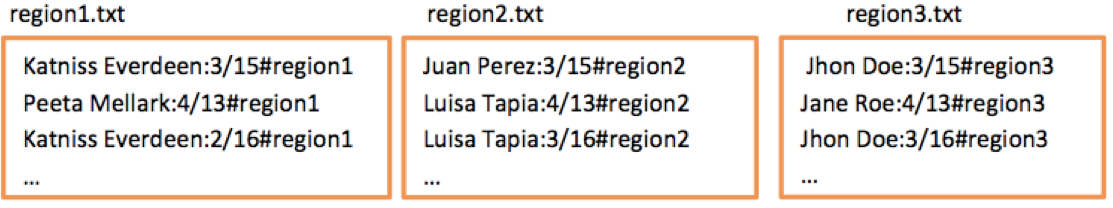
\includegraphics[width=15cm]{Images/i2-1.png}

\textbf{Nota:} Cada archivo puede tener muchos votos

%Por otro lado, el nombre de los archivos de cada zona se encuentra en la lista lista_archivos. lista_archivos = ['region1.txt', 'region2.txt', 'region3.txt']
%Por supuesto, lista_archivos puede tener muchas regiones, no solo las del ejemplo.


\begin{enumerate}
    \item Escriba la función \texttt{juntar\_archivos(lista\_archivos)} que permita generar un archivo llamado \textbf{votaciontotal.txt} con todos los votos de todas las zonas de Chile. La estructura de este nuevo archivo debe ser:
    
    \texttt{Apellido Nombre:región\#factor\_voto}
    Donde \texttt{factor\_voto} se obtiene con la división de la hora por el \texttt{factor\_votante}. La zona se puede obtener por medio del nombre del archivo.
    Ejemplo del archivo \texttt{votaciontotal.txt}\\
    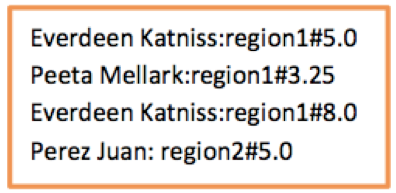
\includegraphics[width=6cm]{Images/i2-2.png}

    \item Escriba una función \texttt{mas\_popular(lista\_archivos)} que genere un archivo que contenga el participante más popular por cada región, el archivo debe quedar de la siguiente forma\\
    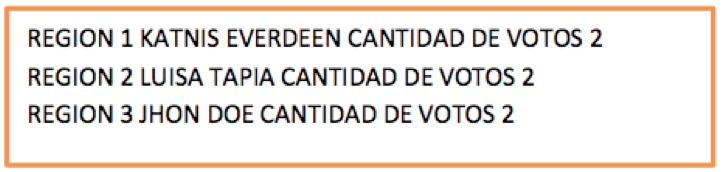
\includegraphics[width=6cm]{Images/i2-3.png}
\end{enumerate}
